\subsubsection*{Methodology of the ASIC subproject.}

\subsubsection*{Electronics and DAQ: the PETSYS solution}
%
\begin{figure}[!htb]
	\centering
	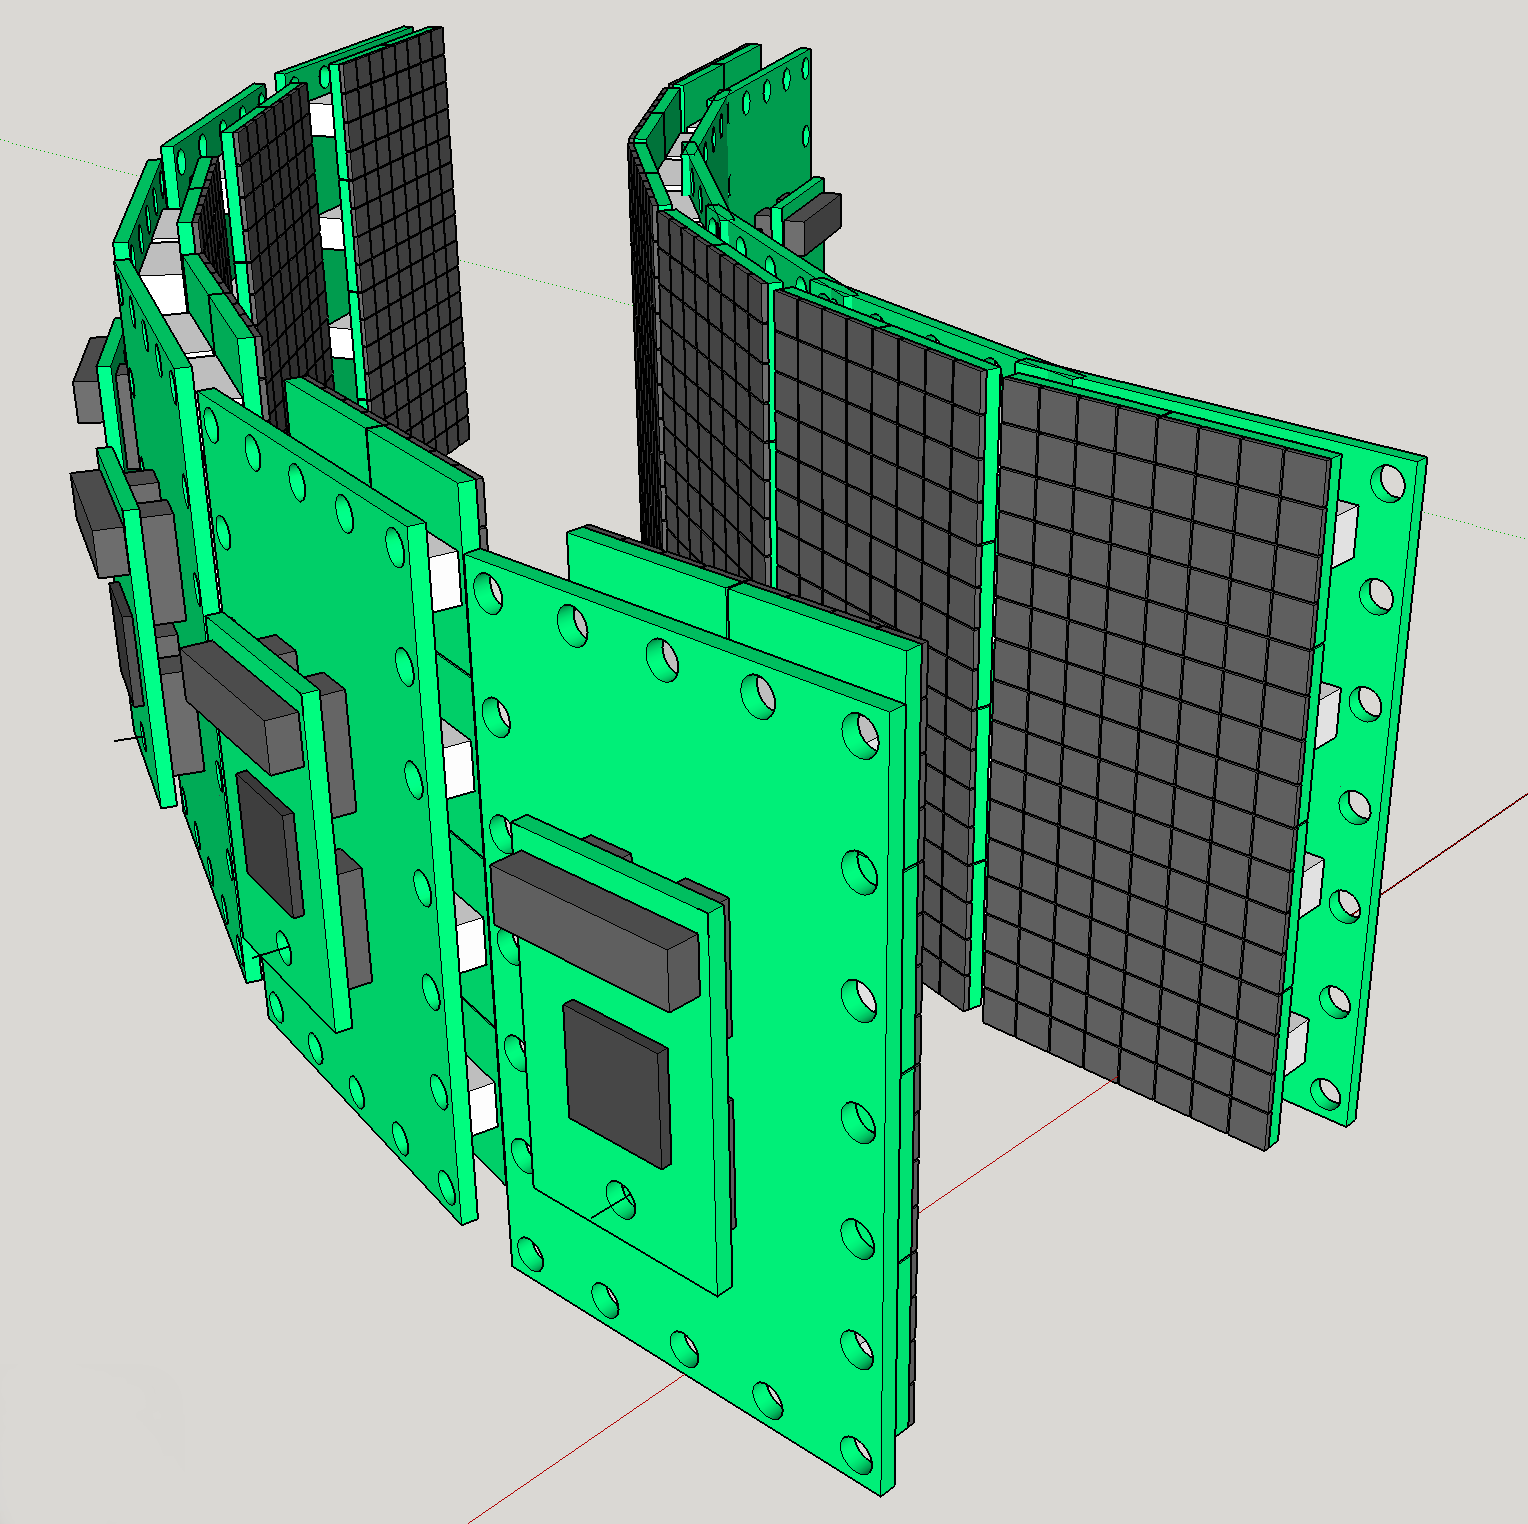
\includegraphics[scale=0.25]{img/PEP.png}
	\caption{\label{fig.pep} A drawing illustrating the arrangement of SiPMs and readout electronics in PEP. }
	\end{figure}

The baseline solution adopted for PETALO is the use of the PETsys TOFPET2 ASIC
\footnote{http://www.petsyselectronics.com/web/website/docs/products/product1/Flyer\%20ASIC\%20TOFPETv2.pdf}, a low power, low noise SiPM readout ASIC
optimised for  time measurement. The ASIC provides signal amplification and discrimination for 64 independent channels. It uses a low threshold
for  timing and a high threshold for accepting the event. Both thresholds are separately configurable for each channel. When any of the 64 channels exceeds the high threshold the ASIC fires, providing a record giving the channel number, the time and the amplitude of the event. The ASIC has large dynamic range (1500 pC) and can handle large
capacitance (thus large SiPMs), offering a SNR of 25 dB for an
input capacitance of 320pF. A fine TDC binning (25 ps) makes it suitable for CRT measurements in the range
of 100 ps. Each channel can handle a hit rate of 600 kHz, the operation frequency is 200 MHz and the max output
rate is 3.2 Gb/s. The output is fully digital and the power consumption around 10 mW/channel.

The crucial features of the ASIC are its low time resolution (25 ps) and the low amplifier noise (25 ps for 1 photoelectron signal).

PETSYS provides a front-end board (FEBA/A) carrying two ASICs, and therefore capable to handle 128 channels. The board dimensions are very compact $52 \times 25.4 \mathrm{~mm^2}$~and fully compatible with the transverse dimensions of the PEP LXSCs ($50 \times 50 \mathrm{~mm^2}$). Thus, each FEB/A can handle a LXSC2 with a double
layer (entry and exit faces) of $8 \times 8$~6 mm SiPMs. If the FEB/A board can be adapted to work at LXe temperatures (it has currently been tested to work at $-80\,^{\circ}{\rm C}$), this allows a very compact readout solution,
as sketched in figure \ref{fig.pep}. Alternatively, one can extract the analog signals of each LXSC using feedthroughs, which have been already developed in the context of the NEXT experiment.

PEP will deploy 14 LXSCs, instrumented with a single DB-A per cell. Each FEB/A can readout two DBs and therefore 7 FEB/A are needed for the whole system. The low power of the ASIC (about 130 mW per FEB/A) results in a total power dissipation of less than 1 W for the whole system, which is much less of the typical power of a standard cryocooler (about 30 W).

The FEB/A digital signals are routed to a concentrator board called FEB/D. A single FEB/D can handle up to 8 FEB/A (thus we need only one FEB/D for PEP). In turn, the FEB/D board sends data to a DAQ master board that can handle up to 12 FEB/D master boards (a master FEB/D, in turn, can daisy-chain several slave FEB/D cards). Thus, the advantage of the solution offered by PETSYS is that is fully scalable to a large system. This would permit a quick upgrade of PEP towards a commercial/pre-commercial system as an spinoff of this project.

The ASIC subproject will contribute to P2 and PEP fabricating and testing the needed DBs for both prototypes. ASIC is also in charge of procuring, testing and commissioning the PETSYS FEE electronics and DAQ. In addition, ASIC will develop the slow controls of the cryogenic and gas systems.

\subsubsection*{Developing electronics suitable for LXe temperatures}

The reliable operation of electronic systems below the military temperature range also known as low temperature electronics (LTE) is quite a challenging objective in itself. Although LTE exploits some useful effects at the device level which enhance the performance of some key components \footcite{fast_lte_dram} there are some severe drawbacks related to reliability at the package and printed circuit board (PCB) which must be carefully studied.
LTE physics in general show a good behavior of some key parameters in microelectronic processes which improve MOSFET devices characteristics. For instance the carrier's mobility increases with lower temperatures which turns into lower channel resistance. Moreover the saturation velocity which is of main importance in deep submicron device transconductance, gets increased in LXe temperature range \footcite{sat_velocity}. Also leakage current gets reduced in LTE which can have a serious impact in high precision detectors. However the reduction of channel resistance also bears a dangerous side effect, the probability of hot electron trapping in the gate interphase rises. This could lead to a premature aging of the transistors and a wide deviation in analog amplifier characteristics. 
PEP and even PETALO will have to put up with periodical thermal cycles for maintenance and trimming at the development stage and also at the final clinical operation. The mismatch of thermal expansion coefficients of the materials at different points of the electronic circuitry \footcite{lau2012thermal} creates mechanical stress which turns into an accelerated aging, fatigue and even failure. This may happen in the die-package adhesive or soldering for flip-chip solutions but also in the wirebonding in case a direct PCB-die bonding is employed in the DB modules. The same failure mechanism can be observed at the PCB level were the thermal stress can be even worse due to the bigger dimensions. The research team foresees a DB and FEB/A redesign taking into account the thermal stress constraints if they are to be placed inside the sealed container.

\subsubsection*{Studies of fast detectors and electronics: collaboration with CLUES}

As discussed in this proposal, the fast and copious scintillation in LXe may allow a CRT in the vicinity of 70-80 ps. The contribution to the CRT comes in part from the effect of the decay constants and the LXe refraction index (that would result in about 50 ps using the first photoelectron) and the response of detectors (e.g, the intrinsic jitter of a SiPM, which is of the order of 100 ps rms) and electronics (about 30--50 ps rms). In LXe there one could also attempt to use the rather copious Cherenkov light (about 100-200 photons per event, typically oner order of magnitude more than in solid scintillators) to reduce the intrinsic contribution to the CRT from $\sim$50 ps to  $\sim$10 ps. In any case, both the detection of Cherenkov light and scintillation light would benefit from developing fast detectors and electronics, contributing with at most 10 ps to the CRT.

Current photo detection technology needs to progress in order to exploit the fast scintillation and even faster Cherenkov prompt emission light. Progress is required in three aspects:
\begin{enumerate}
\item The intrinsic single photon time resolution must be close to the 10 ps rms level.
\item A good PDE ($\sim$ 30 \%) has to be achieved in the UV range to exploit the scarce Cherenkov emission (and would improve very much the response of scintillation). 
\item The Front End (FE) electronics must preserve the timing properties while considering
system design aspect such power consumption and scalability.
\end{enumerate}


The single photon time resolution (SPTR), i.e. the timing jitter measured when one photon is being detected, is an important feature of photo detectors. Photomultiplier tubes (PMT) have typically a SPTR between few hundreds picosenconds and a few nanoseconds. SiPMs achieved SPTR of about 100 ps rms. Micro channel plate PMTs, or MCPs are currently the best sensor to obtain the best timing at single photon level. A promising MCP is being developed by the TORCH project \footnote{T. Gys et al., ``Performance and lifetime of micro-channel plate tubes for the TORCH detector'', NIM A, 766, 2014(171--172).}. An excellent SPTR $\sim$30 ps rms has been measured. Moreover, its sensitivity is already enhanced since it is designed to detect Cherenkov light. Other MCPs present excellent timing (around 30 ps rms) as well\footnote{M. Akatsu et al., ``MCP timing properties for single photons'', NIM A 528 (2004) 763.}.
Furthermore, the Large Area Picosecond Photodetector (LAPPD) collaboration \footnote{B.W. Adams at al.,``Timing characteristics of Large Area Picosecond Photodetectors'', Nucl. Instr. and Meth. A, Vol 795, 2015.} was formed to develop techniques for making large MCP systems.
 
Although MCPs are good candidates to develop a detector with SPTR at the level of 10 ps rms the next key element is the FE electronics which must be customised and optimised for the application. 

The main scientific goal of project CLUES is a proof of a photo-detection scalable module with SPTR of about 30 ps. When operated in coincidence these scalable modules must achieve a CTR better than 50 ps FWHM and a spatial resolution better than 2 mm.

CLUES considers two targets applications: a PET based on Cherenkov radiator or hybrid crystals, and a
PET based on prompt light emission in LXe detectors. The collaboration between CLUES and PETALO will develop along the second line. The P2 apparatus will be used to test fast detectors (most notably MCPs, but the program will also include SPADs and specific studies of SiPMs with low SPTR) and the associated electronics. Subproject ASIC will contribute to specific developments of the electronics, and both groups will participate in the data taking, analysis and interpretation of results. 
